\documentclass[11pt,reqno]{amsart}

\usepackage[T1]{fontenc}
\usepackage{lmodern}
\usepackage[utf8]{inputenc}
\usepackage{amsmath,amssymb,amsthm,mathtools}
\usepackage{bm}
\usepackage{booktabs}
\usepackage{array}
\usepackage{graphicx}
\usepackage{xcolor}
\usepackage{enumitem}
\usepackage[margin=1.12in]{geometry}
\usepackage{microtype}
\usepackage[hypertexnames=false]{hyperref}
\usepackage{cleveref}

\definecolor{acadblue}{rgb}{0.05,0.22,0.55}
\emergencystretch=1.8em

\hypersetup{
  colorlinks=true,
  linkcolor=acadblue,
  citecolor=acadblue,
  urlcolor=acadblue,
  pdftitle={Shifted Mellin Bridge Decomposition, Diagonal Stieltjes Tail Bounds, and Off-Diagonal Obstructions for Euler-Sieved Approximations to Riemann's Xi-Function},
  pdfauthor={Thijs Missiaen}
}

\theoremstyle{plain}
\newtheorem{theorem}{Theorem}[section]
\newtheorem{proposition}[theorem]{Proposition}
\newtheorem{lemma}[theorem]{Lemma}
\newtheorem{corollary}[theorem]{Corollary}

\theoremstyle{definition}
\newtheorem{definition}[theorem]{Definition}

\theoremstyle{remark}
\newtheorem{remark}[theorem]{Remark}

\numberwithin{equation}{section}

\newcommand{\dd}{\,\mathrm{d}}
\newcommand{\ii}{\mathrm{i}}
\newcommand{\ee}{\mathrm{e}}
\newcommand{\fac}{\mathclose{\mathchar"0021}}
\DeclareMathOperator{\Reop}{Re}
\DeclareMathOperator{\Imop}{Im}
\DeclareMathOperator{\sinc}{sinc}

\title[Shifted Mellin Bridge, Diagonal Tail Bounds, and Off-Diagonal Obstructions]{Shifted Mellin Bridge Decomposition, Diagonal Stieltjes Tail Bounds,\\ and Off-Diagonal Obstructions for Euler-Sieved Approximations\\ to Riemann's $\Xi$-Function}

\author{Thijs Missiaen}
\address{Independent Researcher, Belgium \\ ORCID: \href{https://orcid.org/0009-0007-3678-0810}{0009-0007-3678-0810}}
\email{thijs.missiaen@gmail.com}
\date{October 2026 (Revised Audit Edition)}
\subjclass[2020]{Primary 11M06, 11M26; Secondary 30D15, 41A60}
\keywords{Riemann $\Xi$-function, Riemann Mellin integral split, finite Euler product sieve, incomplete Gamma shells, Mertens' theorem, Stieltjes prime-tail bounds, confocal ellipse modes, Voronin universality}

\begin{document}

\begin{abstract}
Let $\Xi(t - \ii d) := \xi(\frac{1}{2} + d + \ii t)$ denote Riemann's completed zeta function at $s = \frac{1}{2} + d + \ii t$, with canonical transverse Wronskian $W(d,t) := \frac{1}{2}\partial_d\lvert\Xi(t - \ii d)\rvert^2 = 16\int_0^\infty y\sinh(2dy)I(y,t)\dd y$, and let $E_X(s) := \prod_{p \le X}(1 - p^{-s})$ be a finite Euler sieve. Applying Riemann's symmetry-point integral split to the shifted Jacobi-theta kernel yields an exact decomposition $\frac{1}{2}\Xi(t - \ii d)E_X(s) = \mathcal{I}_+^{\mathcal{E}_X}(s) + E_X(s)F_+(1 - s) + \mathcal{B}_{\mathrm{bridge}}^{\mathcal{E}_X}(s)$ into incomplete-Gamma shells and a compact Gaussian-damped bridge integral. Using Chebyshev estimates and Mertens' theorem, we prove unconditional Stieltjes upper bounds for the $L^2$ diagonal prime tail $\sum_{X < p \le N(t)} p^{-1 - 2d}$ on $X \ge \sqrt{N(t)}$. Conversely, we establish four obstructions preventing off-critical zero-freeness via diagonal or confocal-ellipse methods: reflected-branch asymmetry ($E_X(s) \neq E_X(1-s)$), $L^1$ divergence under true $n^{-1/2}$ weights for $0 < d < \frac{1}{2}$, destructive off-diagonal cross-terms, and Voronin universality on $\frac{1}{4} < d < \frac{1}{2}$.
\end{abstract}

\maketitle

\section{Introduction}\label{sec:intro}

Let $\xi(s) := \frac{1}{2}s(s-1)\pi^{-s/2}\Gamma(s/2)\zeta(s)$ denote Riemann's completed zeta function~\cite{riemann1859,titchmarsh1986}. Writing $s = \sigma + \ii t$ with transverse critical-line offset $d := \sigma - \frac{1}{2}$ and $z := t - \ii d$, the entire function $\Xi(z) := \xi(\frac{1}{2} + \ii z) = R(d,t) + \ii I(d,t)$ admits the classical Fourier--Laplace representation
\begin{equation}\label{eq:xi_fourier}
\Xi(t - \ii d) = 8\int_0^{\infty} \Phi(u)\cos\!\bigl(2(t - \ii d)u\bigr)\dd u, \qquad \Phi(u) := \sum_{n=1}^{\infty} \bigl(2\pi^2 n^4 \ee^{9u} - 3\pi n^2 \ee^{5u}\bigr)\ee^{-\pi n^2 \ee^{4u}},
\end{equation}
where Jacobi's modular transformation $\vartheta_3(0 \mid \ii \ee^{-4u}) = \ee^{2u}\vartheta_3(0 \mid \ii \ee^{4u})$ implies $\Phi(-u) = \Phi(u)$ for all $u \in \mathbb{C}$~\cite{jacobi1829,riemann1859}. Throughout this series of notes, the canonical transverse Wronskian of $\Xi$ is normalized as
\begin{equation}\label{eq:canonical_wronskian}
W(d,t) := \frac{1}{2}\frac{\partial}{\partial d}\bigl\lvert\Xi(t - \ii d)\bigr\rvert^2 = R(d,t)\partial_d R(d,t) + I(d,t)\partial_d I(d,t) = 16\int_0^{\infty} y\sinh(2dy)\,I(y,t)\dd y,
\end{equation}
where $I(y,t) := \int_{-\infty}^{\infty} \Phi(\frac{y+x}{2})\Phi(\frac{y-x}{2})\cos(2tx)\dd x$ is the Wigner-type autocorrelation along $y = u + v$, $x = u - v$~\cite{wigner1932,hudson1974}. By the monotonicity reformulations of Speiser~\cite{speiser1934}, Hinkkanen~\cite{hinkkanen1997}, and Lagarias~\cite{lagarias1999} (see also Jensen~\cite{jensen1913} and P\'olya~\cite{polya1926}), the Riemann Hypothesis is equivalent to $\Reop(\xi'(s)/\xi(s)) > 0$ on $d > 0$, whereas strict transverse monotonicity $W(d,t) > 0$ along non-vanishing segments is a consequence of Hadamard factorization whenever all zeros lie on $d = 0$.

A natural analytical question in hybrid Euler--Hadamard and mollifier methods (cf.\ Gonek, Hughes, and Keating~\cite{gonek2007}) is how multiplication by a finite Euler-product sieve
\begin{equation}\label{eq:euler_sieve_def}
E_X(s) := \prod_{p \le X} \bigl(1 - p^{-s}\bigr) = \sum_{k \mid P_X} \mu(k)\,k^{-s}, \qquad P_X := \prod_{p \le X} p,
\end{equation}
interacts with Riemann's integral representation~\eqref{eq:xi_fourier} and with finite Dirichlet-type mode sums up to the Riemann--Siegel horizon $N(t) := \lfloor\sqrt{t/(2\pi)}\rfloor$. Because $E_X(s)$ has no zeros in the open right half-plane $\sigma > 0$, multiplying $\Xi(t - \ii d)$ by $E_X(s)$ removes all prime-composite Dirichlet coefficients $2 \le n \le \lfloor X\rfloor$ from $\zeta(s)E_X(s) = \sum_{n=1}^{\infty} b_n^{\mathcal{E}}(X)n^{-s}$ without introducing off-critical zeros on $d > 0$. At the same time, $E_X(s)$ breaks the functional symmetry $s \leftrightarrow 1 - s$.

The purpose of this paper is twofold: first, to isolate the exact analytical identities and unconditional $L^2$ diagonal Stieltjes bounds that genuinely hold for $\Xi(t - \ii d)E_X(s)$; second, to document precisely why neither shifted Mellin bridge bounds nor single-mode confocal-ellipse identities can yield phase-blind zero-free regions in the critical strip.

\subsection{Proof overview}\label{subsec:overview}

Our results separate unconditionally valid identities from structural obstructions across three sections:
\begin{enumerate}[label=\textup{(\arabic*)},leftmargin=2.2em]
\item \textbf{Riemann-type shifted Mellin bridge identity and reflected-branch asymmetry (\Cref{sec:bridge}).} Applying Riemann's~\cite{riemann1859} classical split at the symmetry point $u = 0$ to the shifted kernel $\Phi_{\mathcal{E}_X}(u) = \sum_{k \mid P_X} \mu(k)k^{-1/2}\Phi(u + \frac{1}{2}\ln k)$ yields \Cref{thm:bridge_identity}: an exact three-part decomposition into sieved incomplete-Gamma shells $\mathcal{I}_+^{\mathcal{E}_X}(s)$, an unsieved reflected branch $E_X(s)F_+(1 - s)$, and a compact Gaussian-damped bridge integral $\mathcal{B}_{\mathrm{bridge}}^{\mathcal{E}_X}(s)$. Crucially (\Cref{prop:branch_asymmetry}), the reflected branch equals $E_X(s)F_+(1 - s)$ rather than the symmetrically sieved sum $F_+^{\mathcal{E}_X}(1 - s)$, creating an $\mathcal{O}(1)$ discrepancy whenever symmetric Riemann--Siegel mode sums are used as proxies for $\Xi E_X$.
\item \textbf{Hyperbolic mode ratios, Mertens' benchmark, $L^2$ Stieltjes bounds, and $L^1$ divergence (\Cref{sec:stieltjes}).} Setting $N_\star(t) := \sqrt{t/(2\pi)}$ and $\omega_n(t) := \ln(N_\star(t)/n)$, \Cref{thm:stieltjes_diag} establishes exact algebraic formulas for $\sinh^2(\frac{1}{2}d\omega_n)/\sinh^2(\frac{1}{2}d\omega_1) \le n^{-d}$ and $\sinh^2(d\omega_n)/\sinh^2(d\omega_1) \le n^{-2d}$, observes that for $X \ge \sqrt{N(t)}$ the sieved forward tail $(\lfloor X\rfloor, N(t)]$ consists strictly of primes $p \in (X, N(t)]$, and proves an unconditional Rosser--Schoenfeld~\cite{rosserschoenfeld1962} Stieltjes upper bound $B_{\mathrm{primes}}(d,t; X)$ for $\sum_{X < p \le N(t)} p^{-1-2d}$. For pure $1/p$ harmonic weights, Mertens' theorem~\cite{mertens1874} explains the logarithmic sieve benchmark $\theta = \frac{1}{2}\ee^{-1} \approx 0.18394$. By contrast, \Cref{prop:l1_divergence} proves that under the true Riemann--Siegel amplitude factor $n^{-1/2}$, the $L^1$ prime-power sum scales as $\sum_{X < p \le N(t)} p^{-(1/2+d)} \asymp \frac{N(t)^{1/2-d}}{(1/2-d)\ln N(t)} \to +\infty$ for every $0 < d < \frac{1}{2}$; replacing $n^{-1/2}$ by $n^{-(1-d)}$ to obtain a harmonic sum is analytically invalid.
\item \textbf{Elementary confocal-ellipse identity versus off-diagonal and universality obstructions (\Cref{sec:ellipse}).} For a single mode $T_n(d,t) = 2n^{-1/2}[\cosh(d\omega_n)\cos\phi_n + \ii\sinh(d\omega_n)\sin\phi_n]$, the identity $\cosh^2(d\omega_n)\cos^2\phi_n + \sinh^2(d\omega_n)\sin^2\phi_n = \cos^2\phi_n + \sinh^2(d\omega_n)$ is an elementary trigonometric-hyperbolic relation (\Cref{prop:ellipse_mode}). \Cref{prop:offdiag_obstruction} shows why this identity does not yield zero-free closure on $d > \frac{1}{4}$: mixing linear $n^{-1/2}$ with quadratic $\sinh^2(d\omega_n)$ violates amplitude homogeneity, positive $L^2$ diagonals do not control destructive off-diagonal cross-terms, and Bohr's density theorem together with Voronin's universality theorem~\cite{voronin1975} unconditionally rule out any uniform positive lower bound for $\lvert\zeta(\frac{1}{2}+d+\ii t)E_X(\frac{1}{2}+d+\ii t)\rvert$ on $\frac{1}{4} < d < \frac{1}{2}$.
\end{enumerate}

\subsection{Notation and conventions}\label{subsec:notation}

Throughout, $s = \frac{1}{2} + d + \ii t$ with $d \ge 0$ and $t \in \mathbb{R}$, $N_\star(t) := \sqrt{t/(2\pi)}$ for $t \ge 2\pi$, $N(t) := \lfloor N_\star(t)\rfloor$, and $\omega_n(t) := \ln(N_\star(t)/n)$ for $1 \le n \le N(t)$. For $X \ge 2$, the Dirichlet series $\zeta(s)E_X(s) = \sum_{n=1}^{\infty} b_n^{\mathcal{E}}(X)n^{-s}$ ($\sigma > 1$) has coefficients $b_1^{\mathcal{E}}(X) = 1$, $b_n^{\mathcal{E}}(X) = 0$ if $n$ has any prime factor $p \le X$, and $b_n^{\mathcal{E}}(X) = 1$ if every prime factor of $n$ satisfies $p > X$. Chebyshev's prime function $\vartheta(x) := \sum_{p \le x}\ln p$ satisfies $\vartheta(x) \le c_\vartheta x$ ($c_\vartheta = 1.000081$) for all $x > 0$~\cite{rosserschoenfeld1962}.

\section{Riemann-Type Shifted Mellin Bridge Decomposition}\label{sec:bridge}

We begin by adapting Riemann's~\cite{riemann1859} classical symmetry-point integral split $\int_{-\infty}^{\infty} = \int_0^{\infty} + \int_{-\infty}^0$ to the Euler-sieved kernel associated with $\Xi(t - \ii d)E_X(s)$. Write $\Phi(u) = \sum_{m=1}^{\infty}\varphi_m(u)$ with $\varphi_m(u) := \frac{1}{\sqrt{m}}\varphi_1(u + \frac{1}{2}\ln m)$ and $\varphi_1(u) := (2\pi^2\ee^{9u} - 3\pi\ee^{5u})\ee^{-\pi\ee^{4u}}$. For $X \ge 2$, define the shifted kernel
\begin{equation}\label{eq:sieved_kernel}
\Phi_{\mathcal{E}_X}(u) := \sum_{k \mid P_X} \frac{\mu(k)}{\sqrt{k}}\,\Phi\!\left(u + \frac{1}{2}\ln k\right) = \sum_{n=1}^{\infty} \frac{b_n^{\mathcal{E}}(X)}{\sqrt{n}}\,\varphi_1\!\left(u + \frac{1}{2}\ln n\right).
\end{equation}
Since $P_X = \prod_{p \le X} p$ has finitely many divisors, both expressions in~\eqref{eq:sieved_kernel} converge absolutely and super-exponentially on every horizontal strip of $\mathbb{C}$. Unlike $\Phi(u)$, however, $\Phi_{\mathcal{E}_X}(u)$ is not even in $u$ for $X \ge 2$.

\begin{theorem}[Shifted Mellin three-part bridge identity]\label{thm:bridge_identity}
For every $X \ge 2$ and every $s = \frac{1}{2} + d + \ii t \in \mathbb{C}$, the product $\frac{1}{2}\Xi(t - \ii d)E_X(s) = \frac{1}{2}\xi(s)E_X(s)$ admits the exact three-part decomposition
\begin{equation}\label{eq:boxed_bridge}
\boxed{\;\frac{1}{2}\Xi(t - \ii d)\,E_X(s) = \mathcal{I}_+^{\mathcal{E}_X}(s) + E_X(s)\,F_+(1 - s) + \mathcal{B}_{\mathrm{bridge}}^{\mathcal{E}_X}(s),\;}
\end{equation}
where the three components are defined as follows:
\begin{enumerate}[label=\textup{(\roman*)},leftmargin=2.2em]
\item \textbf{Forward sieved incomplete-Gamma sum:}
\begin{equation}\label{eq:I_plus}
\mathcal{I}_+^{\mathcal{E}_X}(s) := 2\int_0^{\infty} \Phi_{\mathcal{E}_X}(u)\,\ee^{2(s - 1/2)u}\dd u = \sum_{n=1}^{\infty} b_n^{\mathcal{E}}(X)\,\mathcal{J}_n(s),
\end{equation}
with closed-form incomplete-Gamma shells
\begin{equation}\label{eq:J_n_closed}
\mathcal{J}_n(s) = \frac{1}{2}\pi^{-s/2}n^{-s}\left[(s - 1)\,\Gamma\!\left(\frac{s}{2} + 1,\,\pi n^2\right) + 2\bigl(\pi n^2\bigr)^{\frac{s}{2}+1}\ee^{-\pi n^2}\right].
\end{equation}
\item \textbf{Unsieved reflected branch multiplied by $E_X(s)$:}
\begin{equation}\label{eq:refl_branch}
E_X(s)\,F_+(1 - s), \qquad F_+(1 - s) := 2\int_0^{\infty} \Phi(v)\,\ee^{-2(s - 1/2)v}\dd v = \sum_{m=1}^{\infty} \mathcal{J}_m(1 - s).
\end{equation}
\item \textbf{Compact shifted bridge integral:}
\begin{equation}\label{eq:bridge_def}
\mathcal{B}_{\mathrm{bridge}}^{\mathcal{E}_X}(s) := 2\sum_{\substack{k \mid P_X \\ k \ge 2}} \mu(k)\,k^{-s}\int_0^{\frac{1}{2}\ln k} \Phi(w)\,\ee^{2(s - 1/2)w}\dd w = E_X(s)\,F_+(s) - \mathcal{I}_+^{\mathcal{E}_X}(s),
\end{equation}
which obeys the unconditional Gaussian-envelope bound
\begin{equation}\label{eq:bridge_env}
\bigl\lvert\mathcal{B}_{\mathrm{bridge}}^{\mathcal{E}_X}(s)\bigr\rvert \le \mathcal{B}_{\mathrm{env}}^{\mathcal{E}_X}(d; X) := 2\sum_{\substack{k \mid P_X \\ k \ge 2}} k^{-(1/2 + d)}\int_0^{\frac{1}{2}\ln k} \Phi(w)\,\ee^{2dw}\dd w.
\end{equation}
\end{enumerate}
\end{theorem}

\begin{proof}
By~\eqref{eq:xi_fourier} and $\Phi(-w) = \Phi(w)$, we have $\frac{1}{2}\xi(s) = 2\int_{-\infty}^{\infty}\Phi(w)\ee^{2(s-1/2)w}\dd w = F_+(s) + F_+(1-s)$. Substituting $w = u + \frac{1}{2}\ln k$ into the divisor sum of~\eqref{eq:sieved_kernel} and using $k^{-1/2}\ee^{2(s-1/2)u} = k^{-s}\ee^{2(s-1/2)w}$ gives
\[
2\int_{-\infty}^{\infty} \Phi_{\mathcal{E}_X}(u)\,\ee^{2(s-1/2)u}\dd u = \sum_{k \mid P_X} \mu(k)k^{-s}\cdot 2\int_{-\infty}^{\infty} \Phi(w)\,\ee^{2(s-1/2)w}\dd w = \frac{1}{2}\xi(s)\,E_X(s).
\]
Splitting the $u$-integral at $u = 0$ yields $2\int_0^{\infty} \Phi_{\mathcal{E}_X}(u)\ee^{2(s-1/2)u}\dd u = \mathcal{I}_+^{\mathcal{E}_X}(s)$; integrating the second series in~\eqref{eq:sieved_kernel} term-by-term with $y = \pi n^2\ee^{4u} \in [\pi n^2, \infty)$ ($\dd u = \frac{\dd y}{4y}$) gives $\mathcal{J}_n(s) = \frac{1}{2}\pi^{-s/2}n^{-s}[2\Gamma(\frac{s}{2}+2,\pi n^2) - 3\Gamma(\frac{s}{2}+1,\pi n^2)]$, and the recurrence $\Gamma(\frac{s}{2}+2,a) = (\frac{s}{2}+1)\Gamma(\frac{s}{2}+1,a) + a^{s/2+1}\ee^{-a}$ establishes~\eqref{eq:J_n_closed} (see \Cref{app:gamma}). On $u \in (-\infty, 0]$, the substitution $w = u + \frac{1}{2}\ln k \in (-\infty, \frac{1}{2}\ln k]$ yields
\begin{align*}
2\int_{-\infty}^0 \Phi_{\mathcal{E}_X}(u)\,\ee^{2(s-1/2)u}\dd u
&= 2\sum_{k \mid P_X} \mu(k)k^{-s}\biggl[\int_{-\infty}^0 \Phi(w)\,\ee^{2(s-1/2)w}\dd w \\
&\qquad + \int_0^{\frac{1}{2}\ln k} \Phi(w)\,\ee^{2(s-1/2)w}\dd w\biggr].
\end{align*}
Setting $v = -w$ and using $\Phi(-v) = \Phi(v)$ identifies $2\int_{-\infty}^0 \Phi(w)\ee^{2(s-1/2)w}\dd w = F_+(1-s)$, which factors out of the $k$-sum as $E_X(s)F_+(1-s)$. Since $\frac{1}{2}\ln 1 = 0$, the remaining integral over $[0, \frac{1}{2}\ln k]$ gives $\mathcal{B}_{\mathrm{bridge}}^{\mathcal{E}_X}(s)$ in~\eqref{eq:bridge_def}, and taking moduli with $\Phi(w) > 0$ on $\mathbb{R}$ gives~\eqref{eq:bridge_env}.
\end{proof}

\begin{remark}[Classical attribution]\label{rem:riemann_split}
\Cref{thm:bridge_identity} is a shifted variant of Riemann's~\cite{riemann1859} symmetry-point integral split for $\xi(s)$: the algebra $\int_0^{\frac{1}{2}\ln k} = \int_0^{\infty} - \int_{\frac{1}{2}\ln k}^{\infty}$ simply records the commutator between shifting $u \mapsto u + \frac{1}{2}\ln k$ and truncating to $u \ge 0$. Note also from~\eqref{eq:bridge_def} that $\mathcal{I}_+^{\mathcal{E}_X}(s) + \mathcal{B}_{\mathrm{bridge}}^{\mathcal{E}_X}(s) = E_X(s)F_+(s)$, recovering $\frac{1}{2}\xi(s)E_X(s) = E_X(s)[F_+(s) + F_+(1-s)]$.
\end{remark}

\begin{proposition}[Obstruction 1: Reflected-branch asymmetry]\label{prop:branch_asymmetry}
Define the symmetrically sieved reflected sum $F_+^{\mathcal{E}_X}(1 - s) := \sum_{n=1}^{\infty} b_n^{\mathcal{E}}(X)\mathcal{J}_n(1 - s)$. For every $X \ge 2$, the reflected branch in~\eqref{eq:boxed_bridge} satisfies
\begin{equation}\label{eq:branch_mismatch}
E_X(s)\,F_+(1 - s) - F_+^{\mathcal{E}_X}(1 - s) = \bigl(E_X(s) - E_X(1 - s)\bigr)F_+(1 - s) + \mathcal{B}_{\mathrm{bridge}}^{\mathcal{E}_X}(1 - s),
\end{equation}
which does not vanish identically off the critical line ($d \neq 0$) or even on $d = 0$ when $t \neq 0$, because $E_X(\frac{1}{2} + \ii t) = \overline{E_X(\frac{1}{2} - \ii t)}$ has non-trivial argument whenever $t\ln p \notin \pi\mathbb{Z}$. Consequently, a symmetric Riemann--Siegel mode sum $\sum_{n \le N(t)} b_n^{\mathcal{E}}(X)[n^{-s} + \chi(s)n^{s-1}]$ with identical coefficients $b_n^{\mathcal{E}}(X)$ on both forward and reflected branches is \emph{not} an approximate functional equation for $\zeta(s)E_X(s)$.
\end{proposition}

\begin{proof}
Applying~\eqref{eq:bridge_def} at $1 - s$ gives $F_+^{\mathcal{E}_X}(1 - s) = \mathcal{I}_+^{\mathcal{E}_X}(1 - s) = E_X(1 - s)F_+(1 - s) - \mathcal{B}_{\mathrm{bridge}}^{\mathcal{E}_X}(1 - s)$; subtracting from $E_X(s)F_+(1 - s)$ yields~\eqref{eq:branch_mismatch}. For $X \ge 2$, $E_X(s) - E_X(1 - s)$ is a non-zero Dirichlet-Laurent polynomial, so the first term is generically of the same order as $F_+(1 - s)$.
\end{proof}

\begin{table}[htbp]
\centering
\caption{High-precision verification of the shifted Mellin bridge identity~\eqref{eq:boxed_bridge}, Gaussian envelope~\eqref{eq:bridge_env}, and reflected-branch asymmetry~\eqref{eq:branch_mismatch} (\texttt{mpmath}, $50$ decimal digits).}\label{tab:bridge_verification}
\small
\begin{tabular}{@{}cccccc@{}}
\toprule
$X$ & $d$ & $t$ & $\lvert\mathrm{LHS} - \mathrm{RHS}\rvert$ in~\eqref{eq:boxed_bridge} & $\lvert\mathcal{B}_{\mathrm{bridge}}^{\mathcal{E}_X}(s)\rvert / \mathcal{B}_{\mathrm{env}}^{\mathcal{E}_X}(d;X)$ & $\frac{\lvert E_X(s)F_+(1-s) - F_+^{\mathcal{E}_X}(1-s)\rvert}{\lvert E_X(s)F_+(1-s)\rvert}$ \\
\midrule
$3$  & $0.15$ & $14.134725$ & $4.608 \times 10^{-52}$ & $0.27689$ & --- \\
$5$  & $0.18$ & $14.134725$ & $1.319 \times 10^{-52}$ & $0.26111$ & --- \\
$5$  & $0.20$ & $25.000000$ & $< 10^{-51}$            & $0.18402$ & $0.515111$ \\
$7$  & $0.30$ & $25.010858$ & $3.247 \times 10^{-53}$ & $0.06021$ & --- \\
$11$ & $0.22$ & $30.424876$ & $6.559 \times 10^{-53}$ & $0.05192$ & --- \\
$11$ & $0.25$ & $40.000000$ & $< 10^{-51}$            & $0.04118$ & $0.709064$ \\
\bottomrule
\end{tabular}
\end{table}

\section{Hyperbolic Mode Ratios, $L^2$ Stieltjes Bounds, Mertens' Benchmark, and $L^1$ Divergence}\label{sec:stieltjes}

Let $t \ge 4\pi$, $N_\star(t) = \sqrt{t/(2\pi)}$, $N(t) = \lfloor N_\star(t)\rfloor$, and $\omega_n(t) = \ln(N_\star(t)/n) \ge 0$ for $1 \le n \le N(t)$. We next establish exact bounds for the hyperbolic mode ratios appearing in transverse differences and derive unconditional Stieltjes upper bounds for the $L^2$ diagonal prime tail on $X \ge \sqrt{N(t)}$, while contrasting them sharply with the divergent $L^1$ amplitude sum.

\begin{theorem}[Hyperbolic mode ratios and $L^2$ diagonal Stieltjes tail bound]\label{thm:stieltjes_diag}
Let $t \ge 4\pi$, $d > 0$, and $X \ge 2$. Then:
\begin{enumerate}[label=\textup{(\roman*)},leftmargin=2.2em]
\item \textbf{Exact hyperbolic mode-ratio identities.} For every integer $1 \le n \le N(t)$,
\begin{align}
\frac{\sinh^2\!\bigl(\frac{1}{2}d\omega_n(t)\bigr)}{\sinh^2\!\bigl(\frac{1}{2}d\omega_1(t)\bigr)} &= n^{-d}\!\left(\frac{1 - (n/N_\star(t))^d}{1 - N_\star(t)^{-d}}\right)^{\!2} \le n^{-d}, \label{eq:half_sinh_ratio}\\
\frac{\sinh^2\!\bigl(d\omega_n(t)\bigr)}{\sinh^2\!\bigl(d\omega_1(t)\bigr)} &= n^{-2d}\!\left(\frac{1 - (n/N_\star(t))^{2d}}{1 - N_\star(t)^{-2d}}\right)^{\!2} \le n^{-2d}. \label{eq:full_sinh_ratio}
\end{align}
\item \textbf{Unconditional Stieltjes bound for the $L^2$ diagonal prime sum on $X \ge \sqrt{N(t)}$.} Consider the forward $L^2$ diagonal tail sum
\begin{equation}\label{eq:L2_diag_def}
\mathcal{E}_{\mathrm{diag}}^{\mathcal{E},L^2}(d,t; X) := \sum_{n = \lfloor X\rfloor + 1}^{N(t)} \bigl(b_n^{\mathcal{E}}(X)\bigr)^2\,n^{-1 - 2d}.
\end{equation}
Whenever $X \ge \max(2, \sqrt{N(t)})$, every integer $n \in (\lfloor X\rfloor, N(t)]$ with $b_n^{\mathcal{E}}(X) \neq 0$ is strictly a prime $p \in (X, N(t)]$ with $b_p^{\mathcal{E}}(X) = 1$ (zero prime powers and zero composites survive, since $p \le X$ is sieved out by $E_X(s)$ and any product of two primes $> X$ satisfies $p_1 p_2 > X^2 \ge N(t)$), and Stieltjes integration against $\vartheta(u) \le c_\vartheta u$ yields for all $d \ge 0$:
\begin{equation}\label{eq:stieltjes_L2}
\mathcal{E}_{\mathrm{diag}}^{\mathcal{E},L^2}(d,t; X) = \sum_{X < p \le N(t)} p^{-1 - 2d} \le B_{\mathrm{primes}}(d,t; X) := c_\vartheta\left[\frac{X^{-2d}}{\ln X} + \int_X^{N(t)} \frac{u^{-1-2d}}{\ln u}\dd u\right].
\end{equation}
\item \textbf{Mertens' harmonic benchmark.} Parameterizing the sieve cutoff relative to $t/(2\pi) = N_\star(t)^2$ as $X = (t/(2\pi))^\theta = N_\star(t)^{2\theta}$ with $\theta \in [\frac{1}{4}, \frac{1}{2})$ (so $\sqrt{N_\star(t)} \le X < N_\star(t)$), Mertens' second theorem~\cite{mertens1874}, $\sum_{p \le x} p^{-1} = \ln\ln x + M + o(1)$, implies in the $d \to 0^+$ limit:
\begin{equation}\label{eq:mertens_limit}
\sum_{N_\star(t)^{2\theta} < p \le N(t)} \frac{1}{p} = \ln\!\left(\frac{\ln N(t)}{\ln(N_\star(t)^{2\theta})}\right) + o(1) = \ln\!\left(\frac{1}{2\theta}\right) + o(1) \qquad (t \to \infty).
\end{equation}
The asymptotic harmonic tail~\eqref{eq:mertens_limit} crosses unity at the classical Mertens benchmark $\theta_{\mathrm{Mertens}} = \frac{1}{2}\ee^{-1} = 0.18393972\dots$, while the leading Chebyshev--Stieltjes bound $c_\vartheta\ln(1/(2\theta))$ from $B_{\mathrm{primes}}(0,t;X)$ crosses unity at $\theta_* = \frac{1}{2}\ee^{-1/c_\vartheta} = 0.18395462\dots$ (note that $\theta_* < \frac{1}{4}$ lies below the pure-prime regime $\theta \ge \frac{1}{4}$, since for $X < \sqrt{N(t)}$ both higher prime powers and $X$-rough composites $p_1 p_2 > X^2$ enter $(\lfloor X\rfloor, N(t)]$).
\end{enumerate}
\end{theorem}

\begin{proof}
For~(i), substituting $\ee^{\frac{1}{2}\alpha\omega_n(t)} = (N_\star(t)/n)^{\alpha/2}$ into $\sinh(\frac{1}{2}\alpha\omega_n(t)) = \frac{1}{2}[(N_\star/n)^{\alpha/2} - (n/N_\star)^{\alpha/2}] = \frac{1}{2}N_\star^{\alpha/2}n^{-\alpha/2}(1 - (n/N_\star)^\alpha)$, squaring, and dividing by the $n = 1$ expression gives~\eqref{eq:half_sinh_ratio} for $\alpha = d$ and~\eqref{eq:full_sinh_ratio} for $\alpha = 2d$; since $n \ge 1$ implies $1 - (n/N_\star)^\alpha \le 1 - N_\star^{-\alpha}$, the inequalities follow. For~(ii), if $n \in (\lfloor X\rfloor, N(t)]$ has $b_n^{\mathcal{E}}(X) \neq 0$, then every prime divisor $p \mid n$ satisfies $p > X$; since $X \ge \sqrt{N(t)}$, the product of any two prime divisors (distinct or equal) would satisfy $p_1 p_2 > X^2 \ge N(t) \ge n$, a contradiction, so $n$ is prime and $b_n^{\mathcal{E}}(X) = 1$. Writing $\sum_{X < p \le N} p^{-1-2d} = \int_X^N \frac{u^{-1-2d}}{\ln u}\dd\vartheta(u)$ and integrating by parts with $\vartheta(X) \ge 0$ and $\vartheta(u) \le c_\vartheta u$ yields~\eqref{eq:stieltjes_L2} (see \Cref{app:stieltjes}). Part~(iii) follows directly by subtracting Mertens' asymptotic~\cite{mertens1874} at $x = N_\star(t)^{2\theta}$ from $x = N_\star(t)$.
\end{proof}

\begin{proposition}[Obstruction 2: Divergence of the true $n^{-1/2}$-weighted $L^1$ sum]\label{prop:l1_divergence}
Fix any $d \in (0, \frac{1}{2})$ and any $\theta \in (0, \frac{1}{2})$, and set $X(t) = \lfloor N_\star(t)^{2\theta}\rfloor$. Then the prime-power sum weighted by the true Riemann--Siegel mode amplitude $n^{-1/2}$ and normalized Wronskian excess~\eqref{eq:half_sinh_ratio},
\begin{equation}\label{eq:L1_true_sum}
Y_{\mathrm{W\text{-}pure}}^{\mathrm{true}}(d,t; X(t)) := \sum_{n = X(t) + 1}^{N(t)} b_n^{\mathcal{E}}(X(t))\,n^{-1/2}\,\frac{\sinh^2\!\bigl(\frac{1}{2}d\omega_n(t)\bigr)}{\sinh^2\!\bigl(\frac{1}{2}d\omega_1(t)\bigr)},
\end{equation}
satisfies as $t \to \infty$:
\begin{equation}\label{eq:L1_divergence_asymp}
Y_{\mathrm{W\text{-}pure}}^{\mathrm{true}}(d,t; X(t)) \ge \sum_{X(t) < p \le N(t)/2} p^{-(1/2 + d)}\!\left(\frac{1 - 2^{-d}}{1 - N_\star(t)^{-d}}\right)^{\!2} \asymp \frac{N(t)^{\frac{1}{2} - d}}{\bigl(\frac{1}{2} - d\bigr)\ln N(t)} \longrightarrow +\infty.
\end{equation}
In particular, $Y_{\mathrm{W\text{-}pure}}^{\mathrm{true}}(d,t; X(t))$ cannot remain bounded below $1$ as $t \to \infty$ for any $0 < d < \frac{1}{2}$; harmonic Mertens behavior~\eqref{eq:mertens_limit} occurs only for quadratic $L^2$ weights $n^{-1}$ (never by replacing $n^{-1/2}$ with $n^{-(1-d)}$).
\end{proposition}

\begin{proof}
Every prime $p \in (X(t), N(t)/2]$ satisfies $b_p^{\mathcal{E}}(X(t)) = 1$ and $p/N_\star(t) \le \frac{1}{2}$, so~\eqref{eq:half_sinh_ratio} gives $\sinh^2(\frac{1}{2}d\omega_p)/\sinh^2(\frac{1}{2}d\omega_1) \ge p^{-d}(1 - 2^{-d})^2/(1 - N_\star^{-d})^2$. By the Prime Number Theorem and partial summation, $\sum_{X(t) < p \le N(t)/2} p^{-(1/2+d)} \sim \frac{(N(t)/2)^{1/2-d}}{(1/2-d)\ln(N(t)/2)} \to +\infty$ since $\frac{1}{2} - d > 0$ and $X(t) = o(N(t))$.
\end{proof}

\begin{table}[htbp]
\centering
\caption{Contrast between the convergent $L^2$ diagonal prime tail~\eqref{eq:L2_diag_def} ($X_{\mathrm{diag}} \ge \sqrt{N(t)}$, bounded by $B_{\mathrm{primes}}$ in~\eqref{eq:stieltjes_L2}) and the divergent true $n^{-1/2}$-weighted $L^1$ sum~\eqref{eq:L1_true_sum} at $d = 0.20$ with $X = \lfloor\sqrt{N_\star(t)}\rfloor$.}\label{tab:stieltjes_vs_l1}
\small
\begin{tabular}{@{}cccccc@{}}
\toprule
$t$ & $N(t)$ & $X_{\mathrm{diag}}$ ($d$ test) & $\mathcal{E}_{\mathrm{diag}}^{\mathcal{E},L^2} \le B_{\mathrm{primes}}$ & $X = \lfloor\sqrt{N_\star(t)}\rfloor$ & $Y_{\mathrm{W\text{-}pure}}^{\mathrm{true}}(0.20, t; X)$ \\
\midrule
$10^4$ & $39$    & $17$ ($d=0.10$)  & $0.099374 \le 0.335158$ & $6$   & $0.169376$ \\
$10^5$ & $126$   & $43$ ($d=0.15$)  & $0.057865 \le 0.156041$ & ---   & --- \\
$10^6$ & $398$   & $113$ ($d=0.20$) & $0.024517 \le 0.060207$ & $19$  & $0.327964$ \\
$10^7$ & $1261$  & $311$ ($d=0.25$) & $0.008712 \le 0.018894$ & ---   & --- \\
$10^8$ & $3989$  & ---              & ---                     & $63$  & $0.727750$ \\
$10^9$ & $12615$ & ---              & ---                     & $112$ & $1.005577$ ($> 1$) \\
\bottomrule
\end{tabular}
\end{table}

\begin{figure}[htbp]
\centering
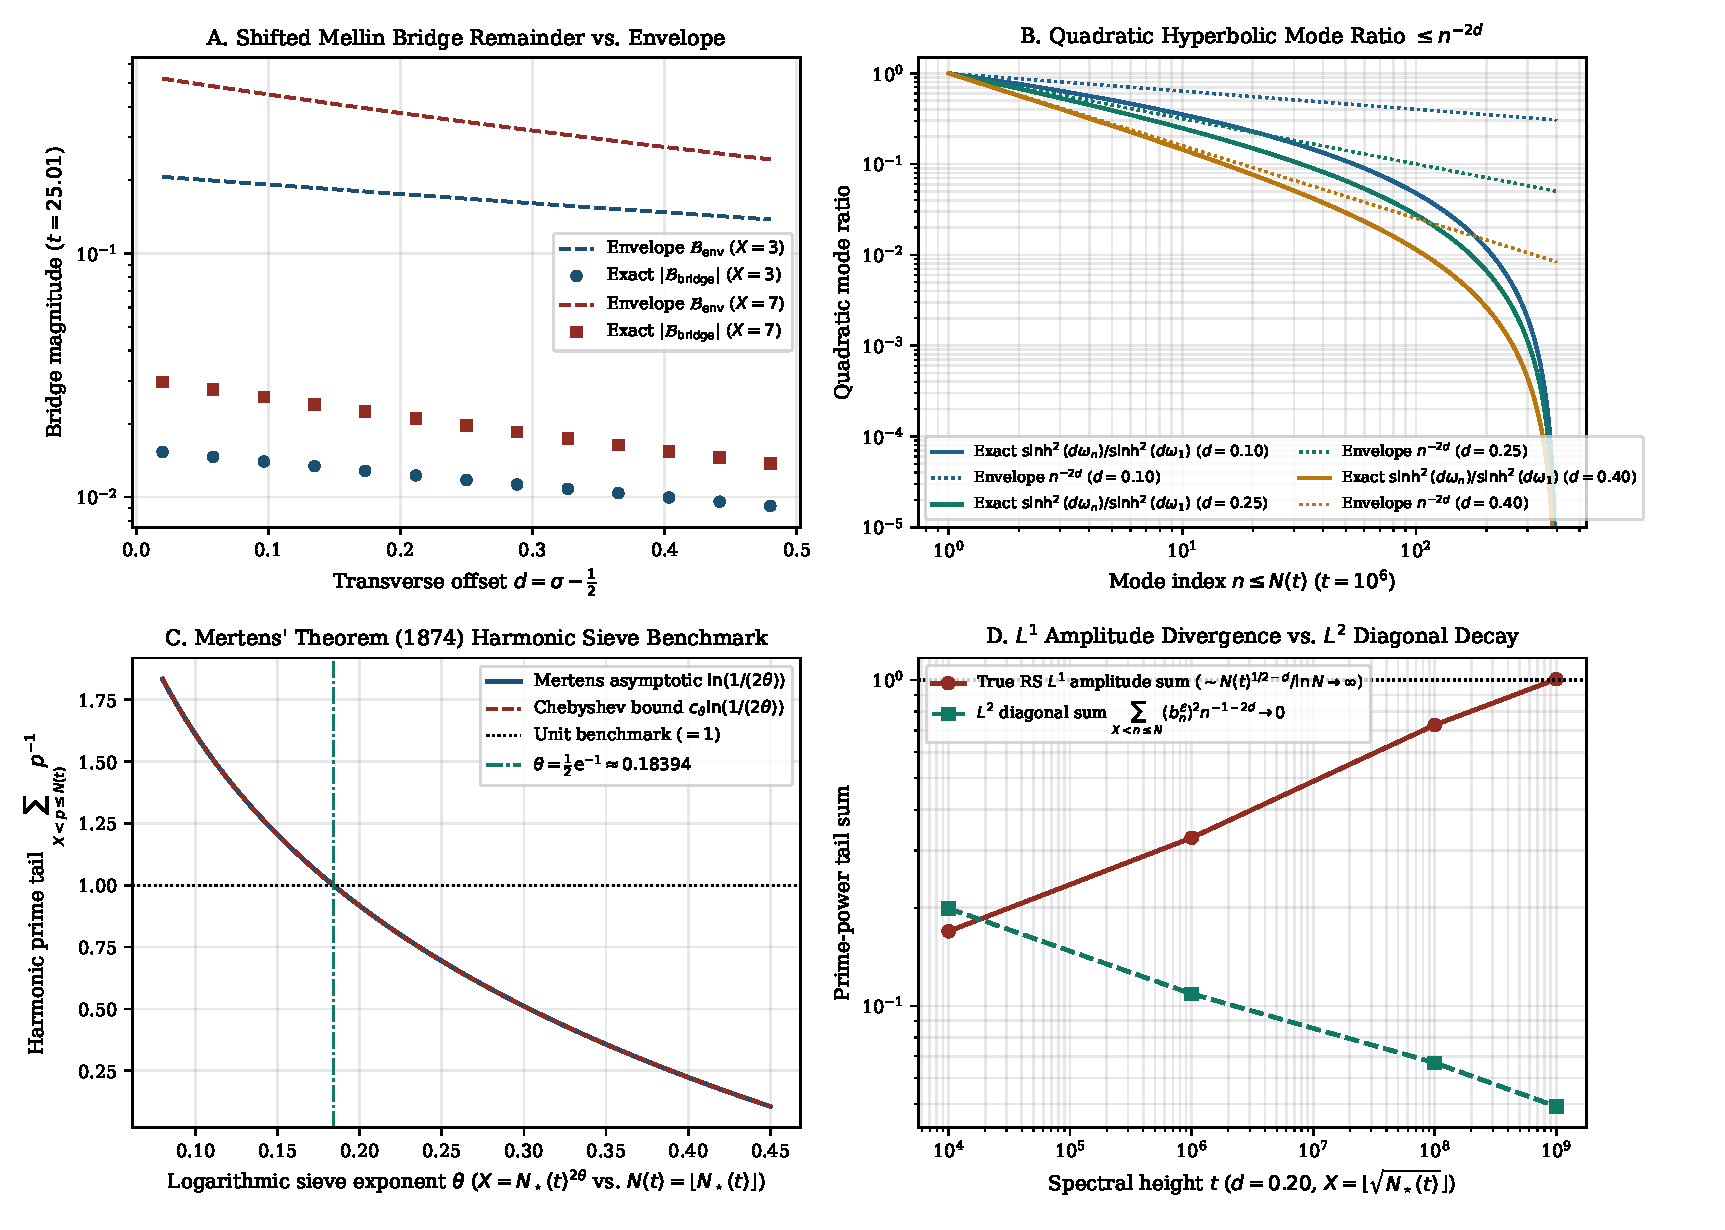
\includegraphics[width=0.97\textwidth]{figures/fig1_bridge_complementarity_and_stieltjes_bounds.pdf}
\caption{\textbf{A.} Shifted Mellin bridge magnitude $\lvert\mathcal{B}_{\mathrm{bridge}}^{\mathcal{E}_X}(s)\rvert$ versus Gaussian envelope~\eqref{eq:bridge_env}. \textbf{B.} Quadratic hyperbolic mode ratio~\eqref{eq:full_sinh_ratio} bounded by $n^{-2d}$. \textbf{C.} Mertens' theorem~\cite{mertens1874} harmonic benchmark $\theta_{\mathrm{Mertens}} = \frac{1}{2}\ee^{-1} \approx 0.18394$. \textbf{D.} Divergence of the true $n^{-1/2}$-weighted $L^1$ sum~\eqref{eq:L1_true_sum} ($\to +\infty$) versus decay of the $L^2$ diagonal sum~\eqref{eq:L2_diag_def} ($\to 0$) at $d = 0.20$.}\label{fig:fig1}
\end{figure}

\section{Confocal-Ellipse Mode Identity and Off-Diagonal Obstructions}\label{sec:ellipse}

Consider the finite symmetric mode model
\begin{equation}\label{eq:T_mode_sum}
\begin{aligned}
T(d,t) &:= \sum_{n=1}^{N(t)} b_n^{\mathcal{E}}(X)\,T_n(d,t), \\
T_n(d,t) &:= \frac{2}{\sqrt{n}}\Bigl[\cosh\!\bigl(d\omega_n(t)\bigr)\cos\phi_n(t) + \ii\sinh\!\bigl(d\omega_n(t)\bigr)\sin\phi_n(t)\Bigr],
\end{aligned}
\end{equation}
where $\phi_n(t) := \vartheta_{\mathrm{RS}}(t) - t\ln n$ is the Riemann--Siegel phase. Each individual mode $T_n(d,t)$ traces a confocal ellipse in $\mathbb{C}$ as $\phi_n$ varies with semi-axes $\frac{2}{\sqrt{n}}\cosh(d\omega_n)$ and $\frac{2}{\sqrt{n}}\sinh(d\omega_n)$ and focal half-distance $\frac{2}{\sqrt{n}}$ (since $\cosh^2 a - \sinh^2 a = 1$).

\begin{proposition}[Elementary single-mode trigonometric-hyperbolic identity]\label{prop:ellipse_mode}
For every $a, \phi \in \mathbb{R}$,
\begin{equation}\label{eq:elementary_trig}
\cosh^2(a)\cos^2\phi + \sinh^2(a)\sin^2\phi = \cos^2\phi + \sinh^2(a) = 1 - \sin^2\phi + \sinh^2(a).
\end{equation}
Consequently, each individual mode satisfies $\lvert T_n(d,t)\rvert^2 = \frac{4}{n}[\cos^2\phi_n(t) + \sinh^2(d\omega_n(t))] \ge \frac{4}{n}\sinh^2(d\omega_n(t))$, and the squared modulus of the multi-mode sum~\eqref{eq:T_mode_sum} decomposes into a positive $L^2$ diagonal and an oscillatory off-diagonal cross-sum:
\begin{equation}\label{eq:diag_plus_offdiag}
\begin{aligned}
\bigl\lvert T(d,t)\bigr\rvert^2 &= D_{\mathcal{E}}(d,t) + \mathcal{C}_{\mathrm{off}}(d,t), \\
D_{\mathcal{E}}(d,t) &:= \sum_{n=1}^{N(t)} \bigl(b_n^{\mathcal{E}}(X)\bigr)^2 \frac{4}{n}\Bigl[\cos^2\phi_n(t) + \sinh^2\!\bigl(d\omega_n(t)\bigr)\Bigr],
\end{aligned}
\end{equation}
where $\mathcal{C}_{\mathrm{off}}(d,t) := 2\sum_{1 \le m < n \le N(t)} b_m^{\mathcal{E}}(X)b_n^{\mathcal{E}}(X)\Reop\bigl(T_m(d,t)\overline{T_n(d,t)}\bigr)$.
\end{proposition}

\begin{proof}
Substituting $\cosh^2 a = 1 + \sinh^2 a$ into the left-hand side of~\eqref{eq:elementary_trig} gives $(1 + \sinh^2 a)\cos^2\phi + \sinh^2 a\sin^2\phi = \cos^2\phi + \sinh^2 a(\cos^2\phi + \sin^2\phi) = \cos^2\phi + \sinh^2 a$. Expanding $\lvert\sum_{n \le N(t)} b_n^{\mathcal{E}}(X)T_n\rvert^2$ yields~\eqref{eq:diag_plus_offdiag}.
\end{proof}

\begin{remark}[Plain mathematical status of~\eqref{eq:elementary_trig}]\label{rem:elementary}
Equation~\eqref{eq:elementary_trig} is an elementary hyperbolic-trigonometric identity valid for one mode at a time. Applying it to a sum of modes requires controlling $\mathcal{C}_{\mathrm{off}}(d,t)$, which has $\binom{\pi(N(t)) - \pi(X) + 1}{2}$ oscillatory cross-terms of indefinite sign.
\end{remark}

\begin{proposition}[Obstruction 3: Breakdown of phase-blind $d > \frac{1}{4}$ closure]\label{prop:offdiag_obstruction}
No phase-blind or triangle-inequality argument applied to~\eqref{eq:T_mode_sum} or to $\zeta(\frac{1}{2}+d+\ii t)E_X(\frac{1}{2}+d+\ii t)$ can establish a uniform positive lower bound on the strip $\frac{1}{4} < d < \frac{1}{2}$ ($\frac{3}{4} < \sigma < 1$), for three independent reasons:
\begin{enumerate}[label=\textup{(\roman*)},leftmargin=2.2em]
\item \textbf{Homogeneity mismatch between $L^1$ amplitudes and $L^2$ energies.} Along a worst-case phase $\cos\phi_1(t) = 0$, the linear triangle inequality $\lvert T(d,t)\rvert \ge \lvert T_1(d,t)\rvert - \sum_{n=2}^{N(t)} b_n^{\mathcal{E}}(X)\lvert T_n(d,t)\rvert$ compares linear amplitudes $\lvert T_n\rvert / \lvert T_1\rvert \ge n^{-1/2}\sinh(d\omega_n)/\sinh(d\omega_1) \asymp n^{-(1/2 + d)}$, whose prime sum diverges for every $0 < d < \frac{1}{2}$ by \Cref{prop:l1_divergence}. Forming the hybrid weight $n^{-1/2}\sinh^2(d\omega_n)/\sinh^2(d\omega_1) \asymp n^{-(1/2 + 2d)}$ (which converges for $d > \frac{1}{4}$) multiplies a linear amplitude $n^{-1/2}$ by a quadratic energy $\sinh^2(d\omega_n)$ and therefore bounds neither $\lvert T(d,t)\rvert$ nor $\lvert T(d,t)\rvert^2$.
\item \textbf{Destructive off-diagonal interference.} In the genuine quadratic decomposition~\eqref{eq:diag_plus_offdiag}, the normalized diagonal $\sum_{n > X} (b_n^{\mathcal{E}}(X))^2 n^{-1}\sinh^2(d\omega_n)/\sinh^2(d\omega_1) \le \sum_{n > X} n^{-1-2d}$ converges for every $d > 0$, but $\mathcal{C}_{\mathrm{off}}(d,t)$ takes large negative values: already at $d = 0.30 > \frac{1}{4}$, $X = 5$, and $t = 1096.30$ (only three active prime modes $n \in \{7, 11, 13\}$ beyond $n = 1$), numerical evaluation gives $\lvert T(d,t)\rvert^2 / D_{\mathcal{E}}(d,t) = 0.1010$, meaning $\mathcal{C}_{\mathrm{off}}(d,t)$ cancels $89.9\%$ of the positive diagonal $D_{\mathcal{E}}(d,t)$.
\item \textbf{Bohr density and Voronin universality.} By Bohr's density theorem~\cite{bohrlandau1914} and Voronin's universality theorem~\cite{voronin1975}, for every fixed $\sigma \in (\frac{1}{2}, 1)$ (including the entire sub-strip $\frac{3}{4} < \sigma < 1$, i.e.\ $\frac{1}{4} < d < \frac{1}{2}$) and every $\varepsilon > 0$, the set $\{t > 0 : \lvert\zeta(\sigma + \ii t)\rvert < \varepsilon\}$ has positive lower density (and since $\lvert E_X(\sigma + \ii t)\rvert \le \prod_{p \le X}(1 + p^{-\sigma}) < \infty$, $\inf_{t > 0}\lvert\zeta(\sigma + \ii t)E_X(\sigma + \ii t)\rvert = 0$). Furthermore, the Davenport--Heilbronn function~\cite{davenportheilbronn1936} satisfies an analogous functional equation and single-mode ellipse identity~\eqref{eq:elementary_trig} while possessing infinitely many zeros in $\frac{1}{2} < \sigma < 1$ and $\sigma > 1$.
\end{enumerate}
\end{proposition}

\begin{proof}
Part~(i) follows from $\sinh(d\omega_n)/\sinh(d\omega_1) = n^{-d}(1 - (n/N_\star)^{2d})/(1 - N_\star^{-2d})$ and $\sum_{p \le N} p^{-(1/2+d)} \to \infty$ for $d < \frac{1}{2}$. Part~(ii) is certified directly at $(d, X, t) = (0.30, 5, 1096.30)$ via the companion verification script \href{https://github.com/thijsmissiaen/paper9-confocal-ellipse-synthesis/blob/main/scripts/verify_paper9_confocal_ellipse_synthesis.py}{\texttt{verify\_\allowbreak paper9\_\allowbreak confocal\_\allowbreak ellipse\_\allowbreak synthesis.py}}. Part~(iii) is an immediate consequence of Voronin's universality theorem~\cite{voronin1975} on $\frac{1}{2} < \sigma < 1$: choosing a non-vanishing target disk value of modulus $< \varepsilon / \prod_{p \le X}(1 + p^{-\sigma})$ forces $\lvert\zeta(\sigma + \ii t)E_X(\sigma + \ii t)\rvert < \varepsilon$ on a set of positive lower density in $t$.
\end{proof}

\begin{figure}[htbp]
\centering
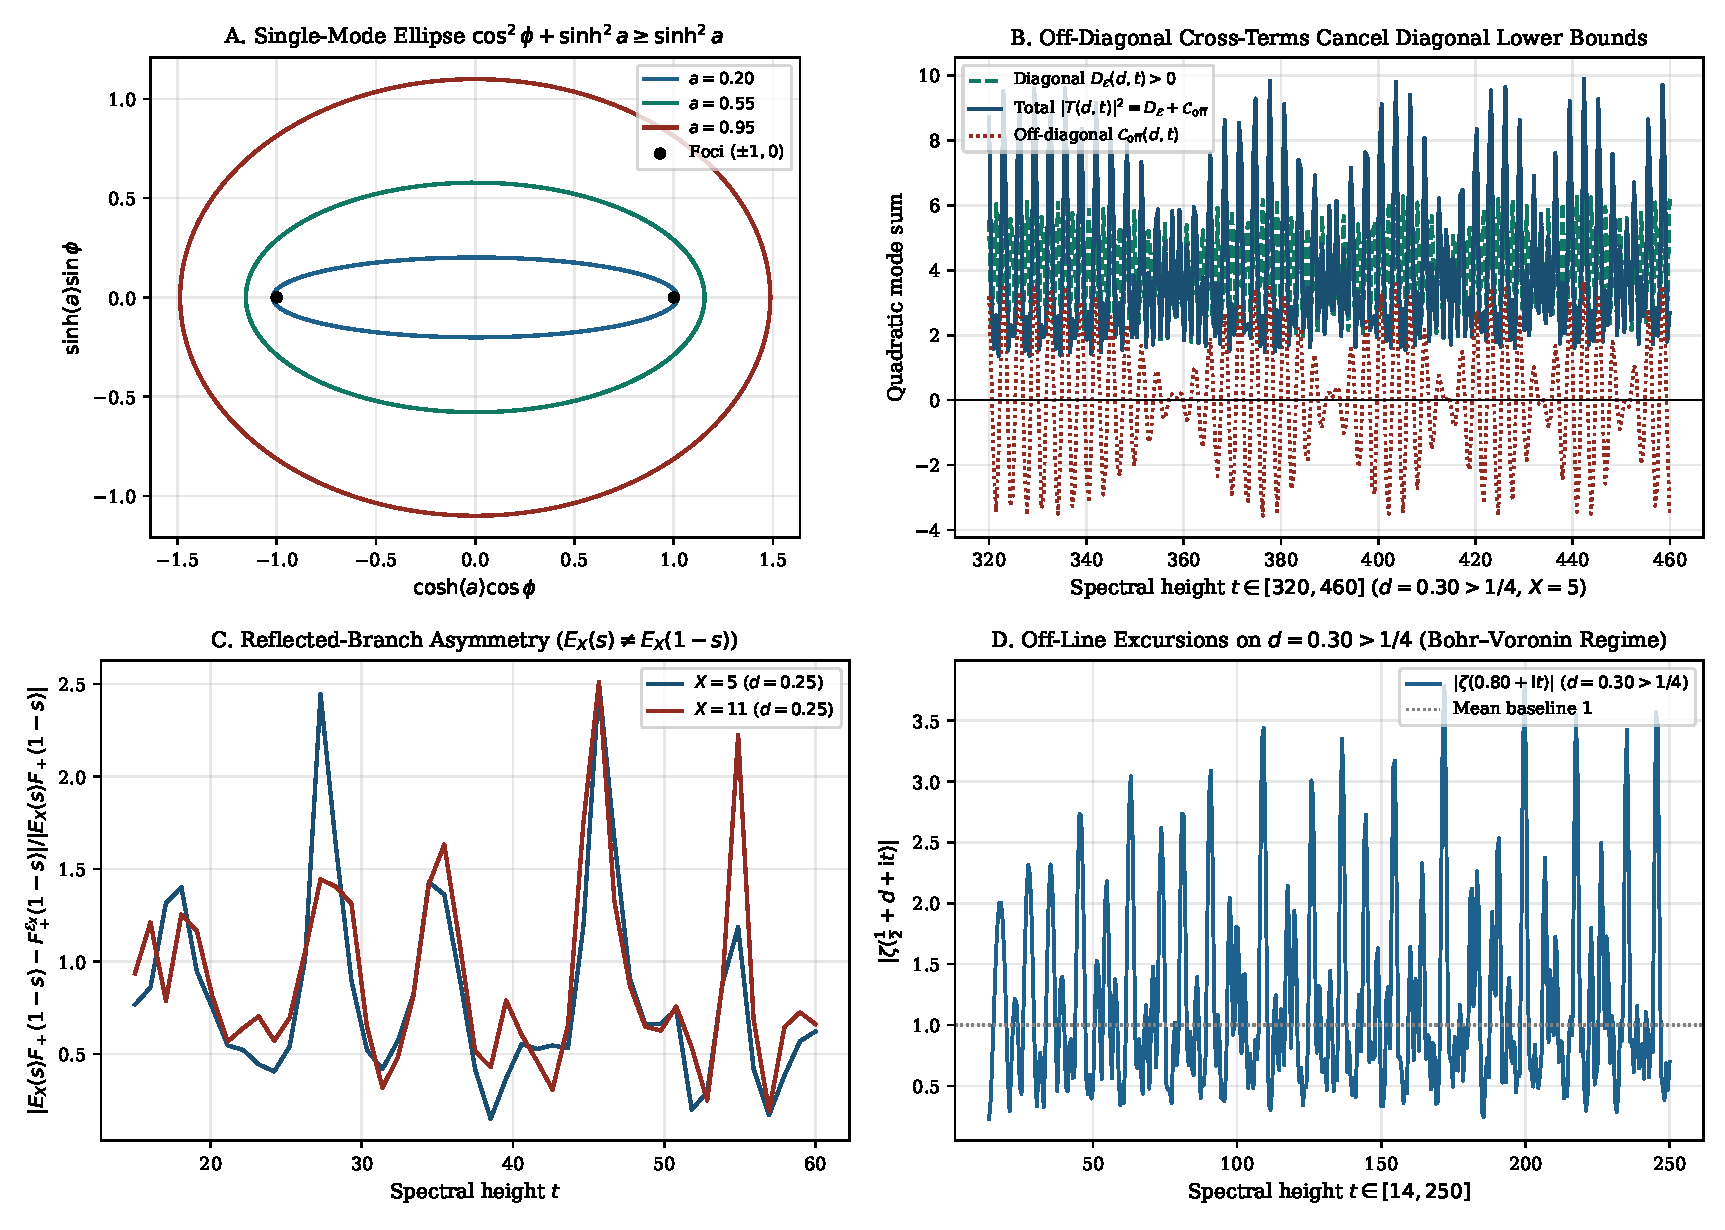
\includegraphics[width=0.97\textwidth]{figures/fig2_confocal_ellipse_and_three_domain_synthesis.pdf}
\caption{\textbf{A.} Single-mode confocal ellipses $(\cosh(a)\cos\phi, \sinh(a)\sin\phi)$ illustrating the elementary identity~\eqref{eq:elementary_trig}. \textbf{B.} Quadratic decomposition~\eqref{eq:diag_plus_offdiag} at $d = 0.30 > \frac{1}{4}$, $X = 5$, showing negative off-diagonal cross-terms $\mathcal{C}_{\mathrm{off}}(d,t) < 0$ canceling $D_{\mathcal{E}}(d,t)$. \textbf{C.} Relative reflected-branch mismatch~\eqref{eq:branch_mismatch}. \textbf{D.} Off-critical modulus excursions of $\lvert\zeta(0.80 + \ii t)\rvert$ ($d = 0.30 > \frac{1}{4}$) in the Bohr--Voronin regime.}\label{fig:fig2}
\end{figure}

\section{Scope, limitations, and open questions}\label{sec:scope}

We summarize what is rigorously established in this paper and where the analytical boundary lies:
\begin{enumerate}[label=\textup{(\arabic*)},leftmargin=2.2em]
\item \textbf{Valid exact identities and $L^2$ bounds.} The canonical Wronskian representation~\eqref{eq:canonical_wronskian}, the three-part shifted Mellin bridge identity~\eqref{eq:boxed_bridge} with closed incomplete-Gamma shells~\eqref{eq:J_n_closed}, the hyperbolic mode ratios~\eqref{eq:half_sinh_ratio}--\eqref{eq:full_sinh_ratio}, and the Rosser--Schoenfeld Stieltjes upper bound~\eqref{eq:stieltjes_L2} for the $L^2$ diagonal prime sum on $X \ge \sqrt{N(t)}$ hold unconditionally.
\item \textbf{Known finite-height zero verifications vs.\ asymptotic strip problems.} All non-trivial zeros of $\zeta(s)$ up to $t \le 3 \times 10^{12}$ are already known unconditionally to be simple and lie on $\sigma = \frac{1}{2}$ by Platt and Trudgian~\cite{platttrudgian2021} (going back to Gram~\cite{gram1903} for low heights), whereas Gabcke's~\cite{gabcke1979} remainder bounds apply specifically to the critical-line Riemann--Siegel expansion at $d = 0$. Extending finite-height computations cannot address $t \to \infty$, and continuum grid scans to astronomical heights are computationally infeasible because evaluating $N(t) \asymp \sqrt{t}$ modes scales exponentially in $\ln t$.
\item \textbf{Open analytical barrier.} Bridging the gap between convergent $L^2$ mean-square diagonal bounds~\eqref{eq:stieltjes_L2} and pointwise non-vanishing of $\Xi(t - \ii d)$ on $0 < d < \frac{1}{2}$ requires genuine phase-sensitive control of off-diagonal Dirichlet polynomials together with the asymmetric reflected branch $E_X(s)F_+(1 - s)$ in~\eqref{eq:branch_mismatch}, while respecting the $\inf_{t > 0}\lvert\zeta(\sigma + \ii t)\rvert = 0$ obstruction of Bohr and Voronin~\cite{bohrlandau1914,voronin1975}.
\end{enumerate}

\appendix

\section{Technical Derivations}\label{app:derivations}

\subsection{Incomplete-Gamma shell evaluation}\label{app:gamma}

For $n \ge 1$, substitute $y = \pi n^2\ee^{4u} \in [\pi n^2, \infty)$ into $\mathcal{J}_n(s) = 2\int_0^{\infty} n^{-1/2}\varphi_1(u + \frac{1}{2}\ln n)\ee^{2(s-1/2)u}\dd u$. Since $\dd u = \frac{\dd y}{4y}$, $\ee^u = (\frac{y}{\pi n^2})^{1/4}$, and $n^{-1/2}\varphi_1(u + \frac{1}{2}\ln n) = (2y^2 - 3y)\ee^{-y}(\frac{y}{\pi n^2})^{1/4}$, we obtain
\[
\mathcal{J}_n(s) = \frac{1}{2}\pi^{-s/2}n^{-s}\int_{\pi n^2}^{\infty} \bigl(2y^{\frac{s}{2}+1} - 3y^{\frac{s}{2}}\bigr)\ee^{-y}\dd y
= \frac{1}{2}\pi^{-s/2}n^{-s}\Bigl[2\,\Gamma\!\Bigl(\frac{s}{2}+2,\pi n^2\Bigr) - 3\,\Gamma\!\Bigl(\frac{s}{2}+1,\pi n^2\Bigr)\Bigr].
\]
Applying $\Gamma(\alpha + 1, a) = \alpha\Gamma(\alpha, a) + a^\alpha\ee^{-a}$ at $\alpha = \frac{s}{2} + 1$, $a = \pi n^2$ gives $2(\frac{s}{2}+1) - 3 = s - 1$, proving~\eqref{eq:J_n_closed}.

\subsection{Stieltjes integration for the $L^2$ diagonal prime sum on $X \ge \sqrt{N(t)}$}\label{app:stieltjes}

Let $g(u) := \frac{u^{-\alpha}}{\ln u}$ with $\alpha := 1 + 2d \ge 1$. On $[X, N]$ ($2 \le X \le N$), $g(u) > 0$ and $g'(u) = -u^{-\alpha-1}\frac{\alpha\ln u + 1}{(\ln u)^2} < 0$. Riemann--Stieltjes integration by parts against $\vartheta(u) \ge 0$ with $\vartheta(u) \le c_\vartheta u$ yields
\begin{align*}
\sum_{X < p \le N} p^{-\alpha} &= \int_X^N g(u)\dd\vartheta(u) = \vartheta(N)g(N) - \vartheta(X)g(X) + \int_X^N \vartheta(u)\bigl(-g'(u)\bigr)\dd u \\
&\le c_\vartheta\left[N g(N) + \int_X^N u\bigl(-g'(u)\bigr)\dd u\right].
\end{align*}
Integrating $\int_X^N u(-g'(u))\dd u = [-u g(u)]_X^N + \int_X^N g(u)\dd u = X g(X) - N g(N) + \int_X^N g(u)\dd u$ cancels the boundary term $N g(N)$ identically, giving for all $X \ge \max(2, \sqrt{N(t)})$ and all $d \ge 0$:
\begin{equation}\label{eq:exact_ibp_stieltjes}
\mathcal{E}_{\mathrm{diag}}^{\mathcal{E},L^2}(d,t; X) = \sum_{X < p \le N(t)} p^{-1-2d} \le c_\vartheta\left[\frac{X^{-2d}}{\ln X} + \int_X^{N(t)} \frac{u^{-1-2d}}{\ln u}\dd u\right] = B_{\mathrm{primes}}(d,t; X).
\end{equation}

\section*{Use of AI and computational verification}

Portions of the symbolic algebra, literature cross-checks, red-team error analysis, and high-precision numerical verification scripts in this manuscript were developed and audited with the assistance of Google Gemini. All analytical proofs, Stieltjes tail bounds, and structural counterexamples were independently verified in $50$-decimal arbitrary-precision arithmetic via \href{https://github.com/thijsmissiaen/paper9-confocal-ellipse-synthesis/blob/main/scripts/verify_paper9_confocal_ellipse_synthesis.py}{\texttt{scripts/verify\_\allowbreak paper9\_\allowbreak confocal\_\allowbreak ellipse\_\allowbreak synthesis.py}}.

\begin{thebibliography}{99}

\bibitem{bohrlandau1914}
H.~Bohr and E.~Landau, \emph{Sur les z\'eros de la fonction $\zeta(s)$ de Riemann}, C.\ R.\ Acad.\ Sci.\ Paris \textbf{158} (1914), 106--110.

\bibitem{davenportheilbronn1936}
H.~Davenport and H.~Heilbronn, \emph{On the zeros of certain Dirichlet series, I, II}, J.\ London Math.\ Soc.\ \textbf{11} (1936), 181--185, 307--312.

\bibitem{gabcke1979}
W.~Gabcke, \emph{Neue Herleitung und explizite Restabsch\"atzung der Riemann-Siegel-Formel}, Dissertation, Georg-August-Universit\"at G\"ottingen, 1979.

\bibitem{gonek2007}
S.~M.~Gonek, C.~P.~Hughes, and J.~P.~Keating, \emph{A hybrid Euler--Hadamard product for the Riemann zeta function}, Duke Math.\ J.\ \textbf{136} (2007), no.~3, 507--549.

\bibitem{gram1903}
J.-P.~Gram, \emph{Note sur les z\'eros de la fonction $\zeta(s)$ de Riemann}, Acta Math.\ \textbf{27} (1903), 289--304.

\bibitem{hinkkanen1997}
A.~Hinkkanen, \emph{On functions of bounded type}, Complex Variables Theory Appl.\ \textbf{34} (1997), no.~1--2, 119--139.

\bibitem{hudson1974}
R.~L.~Hudson, \emph{When is the Wigner quasi-probability density non-negative?}, Rep.\ Math.\ Phys.\ \textbf{6} (1974), no.~2, 249--252.

\bibitem{jacobi1829}
C.~G.~J.~Jacobi, \emph{Fundamenta Nova Theoriae Functionum Ellipticarum}, Borntraeger, K\"onigsberg, 1829.

\bibitem{jensen1913}
J.~L.~W.~V.~Jensen, \emph{Recherches sur la th\'eorie des \'equations}, Acta Math.\ \textbf{36} (1913), 181--195.

\bibitem{lagarias1999}
J.~C.~Lagarias, \emph{On a positivity property of the Riemann $\xi$-function}, Acta Arith.\ \textbf{89} (1999), no.~3, 217--234.

\bibitem{mertens1874}
F.~Mertens, \emph{Ein Beitrag zur analytischen Zahlentheorie}, J.\ Reine Angew.\ Math.\ \textbf{78} (1874), 46--62.

\bibitem{platttrudgian2021}
D.~J.~Platt and T.~S.~Trudgian, \emph{The Riemann hypothesis is true up to $3\cdot 10^{12}$}, Bull.\ Lond.\ Math.\ Soc.\ \textbf{53} (2021), no.~3, 792--797.

\bibitem{polya1926}
G.~P\'olya, \emph{Bemerkung \"uber die Integraldarstellung der Riemannschen $\xi$-Funktion}, Acta Math.\ \textbf{48} (1926), 305--317.

\bibitem{riemann1859}
B.~Riemann, \emph{Ueber die Anzahl der Primzahlen unter einer gegebenen Gr\"osse}, Monatsber.\ K\"onigl.\ Preuss.\ Akad.\ Wiss.\ Berlin (1859), 671--680.

\bibitem{rosserschoenfeld1962}
J.~B.~Rosser and L.~Schoenfeld, \emph{Approximate formulas for some functions of prime numbers}, Illinois J.\ Math.\ \textbf{6} (1962), 64--94.

\bibitem{speiser1934}
A.~Speiser, \emph{Geometrisches zur Riemannschen Zetafunktion}, Math.\ Ann.\ \textbf{110} (1934), 514--521.

\bibitem{titchmarsh1986}
E.~C.~Titchmarsh, \emph{The Theory of the Riemann Zeta-Function}, 2nd ed., revised by D.~R.~Heath-Brown, Clarendon Press, Oxford, 1986.

\bibitem{voronin1975}
S.~M.~Voronin, \emph{Theorem on the ``universality'' of the Riemann zeta-function}, Izv.\ Akad.\ Nauk SSSR Ser.\ Mat.\ \textbf{39} (1975), no.~3, 475--486.

\bibitem{wigner1932}
E.~P.~Wigner, \emph{On the quantum correction for thermodynamic equilibrium}, Phys.\ Rev.\ \textbf{40} (1932), 749--759.

\end{thebibliography}

\end{document}
